\documentclass[11pt]{article}
\renewcommand{\baselinestretch}{1.8}
\usepackage{textcomp}
\usepackage{fontenc}
\usepackage{graphicx}
\usepackage{caption} % for Fig. captions
\usepackage{gensymb} % for \degree
\usepackage{placeins} % for \images
\usepackage[margin=1in]{geometry} % to set margins
\usepackage{setspace}
\usepackage{lineno}
%\usepackage{cite}
\usepackage{amssymb} % for math symbols
\usepackage{amsmath} % for aligning equations
\usepackage[sort&compress]{natbib}
\usepackage{xr-hyper}


\bibliographystyle{..//refs/styles/newphyto.bst}

\linenumbers


\title{Differential sensitivity to the environment between flower and leaf buds drive phenological sequence variation in woody plants\\
or\\
The physiology of flower-leaf sequences in deciduous woody plants: differential sensitivity to the environment drives long-term variation and future shifts with climate change}

\date{}
\author{D.M. Buonaiuto $^{1,2,a}$, E.M. Wolkovich$^{3}$}

\begin{document}
\maketitle
\section*{Abstract}
The order and duration of vegetative and reproductive phenological growth in the spring is an important fitness character for deciduous woody plants in the temperate zone. These flower-leaf sequences (FLSs) appear to be shifting with climate change, but the magnitude and impact of future shifts are difficult to predict without an improved understanding of the phenological coordination between flower and leaf buds with each other and the environment. We used long term field observations and growth chamber manipulations to characterize the phenological responses of flower and leaf buds to variable climate conditions for a suite of temperate woody species. We found that flower and leaf buds respond with differential sensitivity to temperature and day length, and that these differences dictate the direction and magnitude of FLS shifts with climate change. The potential for FLS shifts vary across species, and are likely to compromise the reproductive performance of some wind-pollinated, flowering-first species as global climate continues to change.  %needs work

\section*{Introduction}
\noindent It is well established that phenology, the timing of organisms' life-cycle events and transitions, is a critical biological trait \citep{}. Phenological sequences, the temporal relationships among distinct pheno-phases, also strongly influence plant fitness \citep{Ettinger2018,Savage2019,Chamberlin}. \\

\noindent Among deciduous woody plants, the relative timing of flower and leaf development, or flower-leaf sequences (FLSs), may be particularly consequential to fitness\citep{Gougherty2018}. Flowering prior to 
leaf development is common among species in the temperate zone and this FLS may facilitate efficient pollen transfer for wind-pollinated species \citep{Rathcke_1985}, increase floral visibility in biotically-pollinated taxa \citep{Janzen1967}, improve hydraulic functioning \citep{Gougherty2018,Reich1984} or facilitate early flowering \citep{Primack1987,Savage2019} for species in these regions.

\noindent However climate change is shifting FLSs, suggesting many these critical fuctions may be at risk in the future.   However observed FLS shifts vary among species, which may put some species at greater risk while benefiting others \citep{Buonaiuto2020}.\\ 

\noindent The effects of FLS shifts on woody plant fitness depends on direction and magnitude of the FLS shifts.
\noindent Decades of research suggests that for woody plants in temperate regions, cool winter temperatures (chilling), warm spring temperatures (forcing) and day-length (photoperiod) are the primary drivers of both reproductive and vegetative phenology in the spring \citep{Forrest2018,Flynn2018}. Yet the high levels of inter-annual variation in FLSs and the observed FLS shifts with climate change suggest that there must be differences in how these cues influence phenological activity in floral and leaf buds. Identifying these differences is a necessary step for predicting the direction and magnitude, and ultimately fitness impacts, of FLS shifts with climate change. \\

\noindent In this study, we integrate long-term field observations with experimental climate manipulations to compare the phenological response to changing environmental conditions between flower and leaf buds. We then leverage these data to make generalized projections for how FLSs may shift with future climate change. Finally, we interpret these predictions in the context of the functional hypotheses of FLS variation to assess how FLS shifts may impact the performance of some woody plants.\\  

\subsection*{Physiological hypotheses for FLS variation}
\noindent We are not aware of any previous studies that systematically compare the phenological responses of flower and leaf buds within individuals of wild species. However, because FLS variation has implications for fruit production, several studies have investigated these responses in tree crops \citep[see][]{Guo_2014,Garigalio2016,Citadin2001}. While crop phenology is often quite different than that of even related species wild species, this work in tree crops provides several hypotheses that can serve as starting points for an investigation in wild species.\\

\noindent There are two major hypotheses regarding the underlying physiology that structure FLS variation. Below we briefly review each hypothesis and their predictions for how FLS patterns would be expected to vary or shift in 1) long-term field observations, 2) growth chamber studies, and 3) with climate change.

\subsubsection*{Ordered heat sum requirements}% im making up these names
\noindent Some authors have suggested that reproductive and vegetative buds respond similarly to most environmental cues, but have consistently different forcing requirements for the commencement of phenological activity \citep{Guo_2014}. Under this hypothesis, the first phenophase in the FLS always has a consistently lower heat sum requirement than the second---therefore any observed FLS variation is a product of climate variation during the interphase. This suggests that years in which it is cooler during the interphase heat sums accumulate more slowly, resulting in a longer interphase. Conversely, warmer years should reduce the interphase duration. 

This hypothesis predicts that heat sums during interphase will be consistent (Fig. \ref{fig:field}a) across years, sites, or environmental conditions, even though there may be substantial variation in the duration of the FLS interphase measured in calendar time. Further, the order of phenological events comprising the FLS cannot switch (though the duration of the interphase may vary substantially). At the cue level, ordered heat sums relies on flower and leaf buds sharing the same cues and that photoperiod and chilling cues are very similar in magnitude, but magnitude of the forcing cues, varies such that the second phase in the FLS requires more forcing (the sensitivity ($\delta days/\delta T$) of the second phase in the FLS to forcing should always be higher than the first). When extended to climate change impacts, ordered heat sums predicts that if spring temperatures increase with climate change, FLS interphases will decrease, but never change their sequence.

\subsubsection*{Differential sensitivity to multiple cues}
 \noindent Flower and leaf buds may differ in the strength of their phenological responses to the same environemntal cues. For example, \citet{Garigalio2016} found that in peach cultivars, vegetative buds responded more strongly to chilling exposure and had lower heating requirements than reproductive buds. Given this hypothesis, both the order of phenophases in a given FLS and the duration of the interphase depends on combinations of cues. Generalities regarding FLS variation are more elusive, because forcing, chilling and photoperiod do not perfectly correlate over a growing season. This hypothesis makes several predictions that differentiate it from the ordered heat sums hypothesis:

\noindent \textbf{Field observations:}\\ 1)  There should be substantial inter-annual variation in the duration of the FLS interphase measured in both calendar time and heat sum. (Fig. \ref{fig:field}b).\\ 2) The order of phenophases of FLS may switch among years.\\

\noindent \textbf{Growth chamber manipulations:}\\ 1) Different bud types with have marked differences in their sensitives to each cue environmental cue (Fig. \ref{fig:field}d).\\

\noindent \textbf{Climate change:} While on average the climate is warming, chilling and forcing may increase or decrease at different locations and on different time scales \citep{Ettinger}. Shifts in FLS variation will depend on the direction and rate of change in cues at specific locations and the differential sensitivity of reproductive and vegetative phenology to cue combinations.\\
\section{Methods:}
\subsection*{Data simulations:}
\noindent To better understand how the two hypotheses for FLS physiology would manifest in real data, we performed simple data simulations for each case.  To do...Explain simulations.

\subsection*{Analysis of field observations:}
\noindent We obtained 24 years of phenological data for a suite of woody species growing at Harvard Forest, in Petersham, MA \citep{Okeefe2015} from the Harvard Forest Data Archive (www.website.com).  For each individual tree, we calculated the duration of the FLS interphase in each year by subtracting the calendar day of budburst from the calendar day of flower opening. To calculate the growing degree days of the interphase we obtained daily temperature measurements from the Shaler Meteorological Station at Harvard Forest \citep{}. The temperature data collection at this station ended in 2004, so we only analyzed the phenology data through this season. For each individual tree in each year, we used the R package ``chillR" \citep{} to calculate the Growing Degree Days accumulated during the interphase using a base temperature of 5 \degree C. Because flowers were not observed in all years for all species, we analyzed the data for the seven most well represented species in the dataset. To characterize the interannual variation in the FLS interphase for each of these species, we calculated and the mean and standard deviation interphase length in both calendar time and growing degree days for each year of the data.
\subsection*{Growth chamber study}
\noindent We sampled all plant material used in this experiment from Harvard Forest in Petersham, MA. On October 25, 2016, immediately after most plants in the area entered dormancy but before they could accumulate any significant chilling in the field,  we collected branch cuttings from 7-13 individuals 12 woody plant species (4-12 cutting per individual for a total of 48-56 per species). The species consisted of a mix of deciduous shrubs, understory and canopy trees commonly found in mesic hardwood forests of the eastern United States (see S1 for species list). We transported all cuttings to the the Arnold Arboretum in Boston, MA where they were re-cut in water to prevent callousing and cavitation and place in Erlenmeyer flasks with distilled water.\\ %emw8May2020: 500 ml?

\noindent We randomly assigned cuttings to a full set of eight experimental treatments; 2 levels of chilling (4 vs 8 weeks at 4\degree C), 2 levels of temperature (24\degree C:18\degree C warm vs 18\degree:12\degree C cool) and 2 levels of photoperiod (12 vs 8 hours). We alternated day/night temperature periodicity on a 12 hour schedule to reduce co-variation with photoperiodicty. We re-cut all twig and changed the water every 7-10 days and rotated all treatments between growth chambers every two weeks to minimize chamber effects. We made phenological observations every 2-3 days using the modified BBCH scale for woody plants \citep{} for 3 month following release from chilling conditions. In this period we assess three phenological phases: budbreak (BBCH phase 07), leaf unfolding (BBCH phase 15) and first flower open (BBCH 60). At the conclusion of this period we assessed all individuals that did not undergo budbreak and excluded any dead individuals for analysis.

\subsection*{Analysis of growth chamber study}
%emw8May2020: clarify where your grouping factor is: slopes and intercepts?
\noindent To assess the sensitivity of each phase, we fit mixed-effect hierarchical models with chilling, forcing, photoperiod and all two-way interactions as the fixed effects and species as a random-effect grouping factor. We chose a Bayesian, hierarchical approach in order to identify systematic trends across species' responses while accounting for sample size, variance and the unique effect of each species.\\

%emw8May2020: I think we can cut the below paragraph, as long as we specify the intercept condition in the captions (more useful to specify it there anyway); likewise use of dummy variables should be obvious when looking at model output and figures as long as clearly labeled (e.g., 4 hour difference) 
\noindent Because we applied two levels for each environmental treatment in the experiment, we re-coded each treatment as 0/1 dummy variables to improve model performance, so model intercepts can be interpreted as the predicted phenological response when all treatments are at their lowest level. Given that true zeros for these treatment levels are unrealistic in nature, in addition to computational efficiency, this approach also allows for a realistic interpretation of model intercepts.\\  

\noindent We fit all models using the R package ``brms" \citep{}. We ran each model on four chains with 4000 iterations with a 3000 iteration warm up for a total of 4000 sampling iterations. In both models We used weakly informative priors and increasing the priors 5-fold did not affect the model results.\\

The models we fit appear below:\\
(Write models here)
\subsection*{Climate change predictions}
\noindent To apply our model results to general climate change projections we chose our environmental treatments in this experiment to reflect historic and future conditions at Harvard Forest. Our low forcing treatment approximates average spring temperature (March/April) at the site while our high temperature treatment reflects a 5 \degree C increase. Average field chilling (measured in Utah units) at Harvard Forest is X, approximately 60 \% of the difference between our low and high chilling treatment. Thus, our low chilling treatment represents a feasible estimate for a decrease in chilling with climate change and our high chilling treatment approximate reasonable increase. We should note that our low photoperiod treatment (8 hours of daylight) is well below the photoperiod experienced at Harvard Forest, but given that the photoperiod effects are expected to be small, we chose more extreme values in order to robustly estimate an effect (i.e., increasing statistical power). For this reason, our climate change projections for FLS variation are based on our high photoperiod treatment alone.\\

\noindent We used our flower and budburst models to project for each species in our study:\\
\begin{itemize}
\item The historical range of FLS (low forcing, 60 \% chilling)
\item FLS shifts with spring warming only (high forcing, 60 \% chilling-- equivalent to ~6.5 weeks of chilling treatment)
\item FLS shifts with warming and increased chilling ((high forcing, 100 \% chilling-- equivalent to 8 weeks of chilling treatment)
\item FLS shifts with warming and decreased chilling ((high forcing, 0 \% chilling-- equivalent to 4 weeks of chilling treatment)
\end{itemize}

\noindent Given the variable dynamics of shifts in environmental forcing and chilling with climate change over time and space, these projections should not be treated as absolute predictions of the magnitude of FLS shifts with climate change. Instead, we provide these projections to identify general trends in how FLSs could shift with warming and demonstrate the range of possibilities vary based on individual characteristics of plant species and the specific climate dynamics.\\

\section*{Results}
\subsection*{Field Observations}
We found that for individuals at Harvard Forest both the calendar time and heat sums accumulated during the FLS interphase varied significantly across years. For \texit{Acer rubrum}, the species with the most FLS observations in the data set, the calendar days of the interphase varied from X-Y and GDD of the same period from Z-A \ref{fig:acerub}.\\

\noindent We found that the magnitude of GDD variation during interphase differed among species, but almost all had patterns that were more reflective of the differential sensitivity hypothesis (Fig. \ref{allothers}). We found similar patterns in the interphases of other floral-leaf sub-phases (eg. flower and leaf budburst) and observed that the order of these phenophases switch periodically in some species over time (Fig. \ref{otherphases}) lending further support to the differential sensitivity hypothesis. 

\subsection*{Growth chamber study}
\noindent We found that that flower and leaf buds response to environmental cues with differential sensitivity (Fig. \ref{fig:model}). Specifically, while both bud types had a proportionate response to forcing, leaf buds were more sensitive to chilling. At low levels of chilling and forcing, flower buds tended to advance which increasing photoperiod while leaf buds were delayed. Leaf buds were more sensitive to cue interactions, demonstrating stronger responses to increasing in multiple cues than flower buds. While the order of the FLS remained consistent across treatment combinations in most species, we found that one species, \textit{Vaccinium corymbosum} switched FLS order across chilling treatments (Fig. \ref{fig:raw}). 

\subsection*{Climate change predictions}
\noindent Our model predicted that both flower and leaf phenology will advance in most of our generalized scenarios for most species, but shifts in FLS vary depending on how forcing levels change relative to chilling duration (Fig. \ref{fig:preddy}). As would be expected from the significant differences in sensitivity between flowering and leafing phenology in our model, the FLS interphase was more strongly influenced by changes in chilling exposure than increased forcing alone. The direction and magnitude of shifts in the FLS interphase depended on species and the specifics of FLS order, with flowering-first and concurrent species tending show more profound alterations to FLS patterns than leafing-first ones. Under some warming scenarios, our model predicted that the FLS interphase effectively disappear or the order of phenophases would switch (see Fig. \ref{fig:preddy}b-f).

\section*{Discussion}
\subsubsection*{Outline}
\begin{enumerate}
\item summarize results
\item compare results to crops
\item FLS shifts sensitive to chilling and chilling trends vary by location
\item Integrate magnitude with hypotheses
\begin{itemize}
\item hysteranthous wind pollination and strong shifts- bad outcome
\item synanthous insect pollinated, fairly strong shifts- unclear outcome
\item seranthous insect pollinated, weak shifts
\end{itemize}
\item qualify photoperiod impacts
\end{enumerate}

%emw8May2020: Below is good!
\noindent Our analysis of long term field observations and experimental results suggest that flower and leaf buds are differentially sensitive to the primary environmental cues of spring phenology. Specifically, vegetative buds are more sensitive to chilling and cue interactions, and flower buds more sensitive to photoperiod. This differential sensitivity generates the high level of inter-annual FLS variation observed in nature, and will dictate the direction and magnitude of FLS shifts with climate change.\\

\noindent Our findings in support of the differential sensitivity hypothesis are consistent with much of the tree crop literature. Like studies in peaches \citep{Garigalio20106,Citidin2001} we found that the heat requirements for phenological activity were dictated by cue combinations, with leaf buds responding more strongly to chilling than flower buds. Similarly, we also found that like peaches, flowers in some species (eg \textit{Vaccinium corybosum}) tend to emerge before the leaves at low chilling levels. We found no crop literature that evaluated the differential sensitivity of flower and leaf buds to photoperiod. However, consistent with our findings, genetic work in the model genus \textit{Populus} suggests that flowering may be under stronger photoperiodic control that leafing \citep{}.

\noindent We found that species differ in the direction and magnitude of their FLS shift with variable climate conditions. Several species had FLSs that were relatively robust to changing environments. These species, \textit{Ilex verticillata}, \textit{Prunus pensylvanicum}, \textit{Prunus virginiana}, and \texit{Viburnum acerifolium}, all share a strongly leafing-first FLS, with the  fairly long FLS interphase. These species all also have mixed buds, so there may be relatively strong physiological constraints on their FLS. With climate change, it may be that any functional impacts of FLS shifts specifically will be minor compared to those that come about from phenological shifts in general such as alterations to the growing season \citep{}, increased risk of frost or pest damage \citep{}, and phenological mismatch \citep{}. \\

For all other species, the were significant shifts in FLS under varying climate conditions. The direction and magnitude shifts largely depend on how forcing and chilling shifted relative to each other. In many northern temperate locations, chilling is projected to increase over the next several decades \citep{Ettinger}, while in other locations, it may rapidly decrease. These divergent trajectories are likely to increase the population level variation in FLS.\\

\noindent Importantly, the impact of these FLS shift depends not only on the magnitude of the shift, but also on the adaptive function of FLS, which is also likely to differ between taxa in this study and in temperate forest communities in general. Our study identified several species with significant FLS variation under different treatment conditions and fairly substantial FLS shifts with climate change. For \textit{Acer pensylvanicum}, \textit{Vaccinium corymbosum} and \textit{Ilex mucronata}, which typically begin to produce leaves shortly before flowers open, increased forcing coupled with a reduction in chilling advanced flowering more than vegetative budburst, resulting in a switch to concurrent or flowering-first FLS. The performance implications for such shifts are not clear. If these species rely on visual pollinators, this shift may increase pollination success, but as of yet, there is little evidence for the pollinator visibility hypothesis of FLS. In accordance with the water dynamics hypothesis, this shift could theoretically reduce hydraulic demand on the plant as a whole by partition the phenological activity of these two tissues. However, this emerging flowering-first phenotype may not confer much hydraulic advantage given that our model projects that the FLS interphase would still be very short (a few days) and that it is unlikely that plants are water limited in the spring season in the temperate zone \citep{Polgar2011}.\\

\noindent Shifts in FLS may be most consequential for wind-pollinated taxa. There is growing evidence that a flowering-first FLS is an important adaptation for wind pollination, reducing barriers for airborne pollen transfer\citep{Rathcke_1985}. For example, \citet{Tauber1967} quantified the amount of pollen impacted on non-floral structures, estimating that a single branch with leaves would intercept more than double than what was impacted on a bare branch. This suggests that a reduction in the FLS interphase may dramatically reduce reproductive success of flowering-first, wind-pollinated taxa.\\

\noindent In our study, the two species with the most significant FLS shifts across treatment combinations were the flowering-first, wind-pollinated species \textit{Comptonia peregrina} and \textit{Corylus cornuta}. In all of our climate change scenarios, the FLS interphase was dramatically reduced in these taxa. Given the hypothesized function of FLS in wind pollinated species, and the observed direction and magnitude of FLS shifts in our experiment, it may be that these species, and flowering-first, wind-pollinated taxa in general, may face particular risk for reproductive performance reductions from FLS shifts.\\ 

%emw8May2020 -- see my edits below (and check, is just one species an issue? Or both?) ... readers generally don't understand partial pooling so need to explain issue more simply
\noindent However, we did not observed this trend in the other wind-pollinated, flowering first species in our study \textit{Acer rubrum}, which maintained a fairly large and consistent FLS interphase in each of the treatment combinations in our study, as well as in our climate change projections. While the low sample size in our study for these (or this one?) species warrants caution in interepreting this finding, it may reflect biological differences between these species. \textit{Acer rubrum} is a canopy tree while the other two species are low growing, understory shrubs. These species are also phylogenetically distant \citep{}. Additionally, the genus \textit{Acer}, is ambophilous\citep{Dejung_1972}, and there is evidence that even \textit{Acer rubrum} which is considered largely wind-pollinated may still rely on insects for pollination as well \citep{}. These species also have very different floral morphologies (access dejong to describe this better).\\

\noindent The particulars of the floral morphology in \textit{Corylus} and \textit{Comptonia} and their relatives in the temperate dominant Betulaceae, Juglandaceae and Fagaceae, and Salicaece families may further increase the functional impact of FLS shifts. The taxa are generally monoecious and protandrous, with staminate flowers proceeding pistillate ones to promote out-crossing \citep{}.  Staminate flowers are born on separate catkins, while pistillate flowers emerge from within leaf buds and temporally constrained leaf phenology. Thus, a reduction in the FLS interphase correlates with a reduction in dichogamy, increasing the likelihood of self-pollination and ultimately inbreeding depression \citep{}.

\noindent Much of the conversation around phenology and pollination in the context of global change has centered around trophic mismatches between pollinator and floral phenology \citep{}, which is of little relevance to abiotically pollinated taxa. By contrast, we find evidence that the effect of FLS shifts with climate change may be particularly important for abiotically pollinated woody plants and the scope and impact of FLS shifts in these taxa should be explored in greater detail in the future.\\ %emw8May2020 -- last bit here is a very good point! I like it. 

\noindent Despite the fact that on our experiment we found photoperiod to be an important cue dictating FLS shifts, in our FLS projections with climate change we modeled climate change scenarios with a constant photoperiod. Climate change does not directly impact photoperiod, but warming does shift the time of year when plants become phenologically active, changing the photoperiod they experience. However, depending on the latitude, phenology would have to shifts by at minimum several weeks before the experience photoperiod would change substantially \citep{Ettinger}. However, at high latitudes where photoperiod changes more rapidly over the season, the experienced photoperiod may mute FLS shifts captured in our projections. This may be particularly important as species shift shift their distribution poleward with climate change and begin to encounter novel photoperiod regimes \citep{}.\\

\section*{Conclusion:}
Both our field observations and experimental study provide strong evidence that flower and leaf buds integrate the same environmental cues differently, maintaining variation in FLS. As climate change continues to alter these temperature cues, species with physiologically independent buds and strongly divergent temperature sensitivities among bud types will likely experience significant shifts in FLS. This shifts may be particular detrimental to flowering-first, wind-pollinated species that rely on a lengthy leaf-free period for pollination. Because of the prevalence of these taxa in temperate forests. the scope and impact of FLS shifts in these taxa remain a high research priority.\\

\section*{Supplement:}
\begin{enumerate}
\item Species list
\item field plots for extra species
\item table with chilling comparisons
\end{enumerate}
 
\bibliography{..//refs/hyst_outline.bib}
\section{Figures}

\begin{figure}[h!]
\centering
 \includegraphics[width=.8\textwidth,angle =90]{..//Plots/Flobuds_manuscript_figs/simulationfigure.pdf}
   \caption{\textbf{This figure predicts the field (a-b) and experimental (c-d) results under the order heat sums (a\& c) and differential sensitivity (b \& d) hypothesis}}
    \label{fig:field}
\end{figure}

\begin{figure}[h!]
    \centering
 \includegraphics[width=\textwidth]{..//Plots/Flobuds_manuscript_figs/hypothesis1_acerub.jpeg}
    \caption{\textbf{look there is high variation in acer rubrum, also need to remake this figure}}
    \label{fig:acerub}
\end{figure}

\begin{figure}[h!]
    \centering
 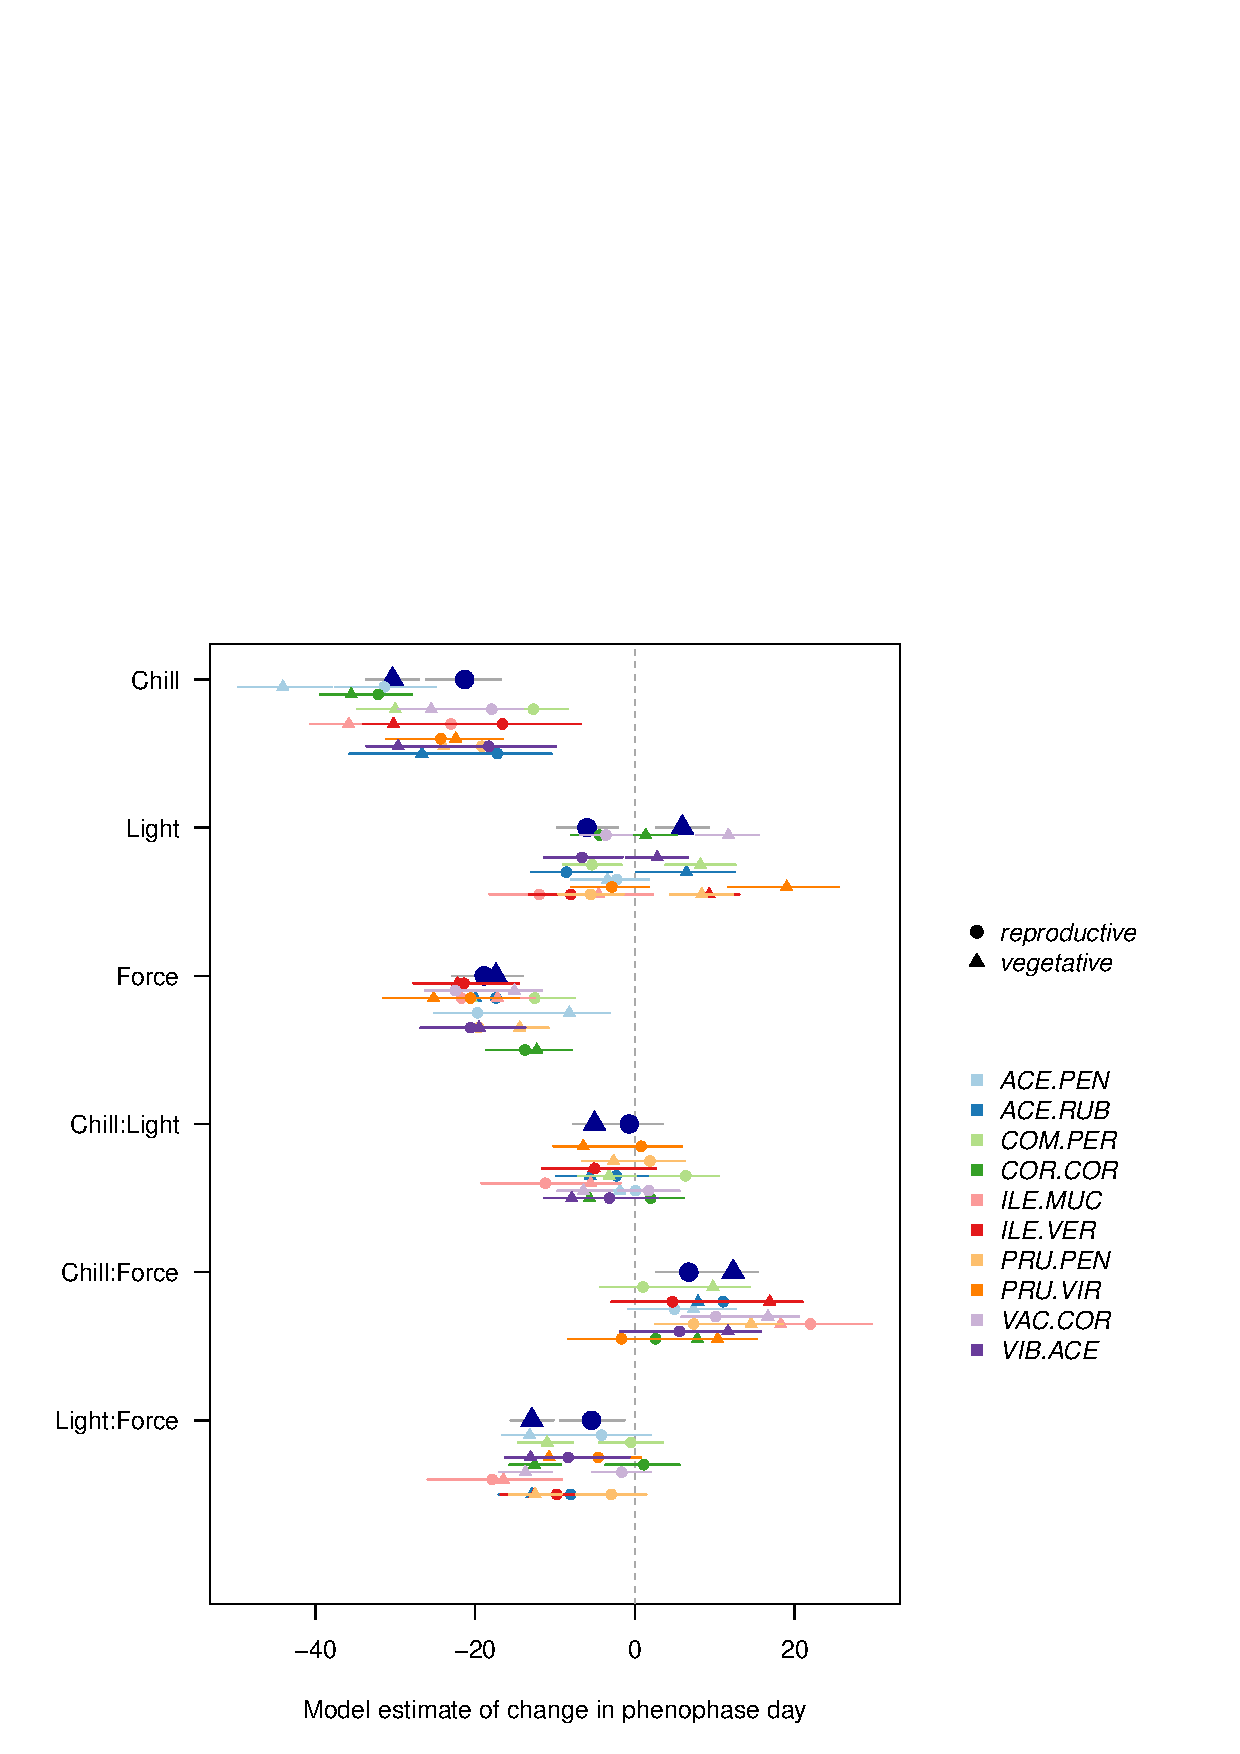
\includegraphics[width=\textwidth]{..//Plots/Flobuds_manuscript_figs/budburstvsflowering.pdf}
    \caption{\textbf{Experimental results suggest differential sensitivity to environmental cues between flower and leaf buds}. Vegetative buds (circles) as more sensitive to chilling and interaction between chilling and forcing. Flower buds (triangles) advance with photoperiods increases but leaf buds appear to delay. These differential sensitivities have implications with how FLS patterns vary given environmental variation}
    \label{fig:model}
\end{figure}

    \begin{figure}[h!]
    \centering
 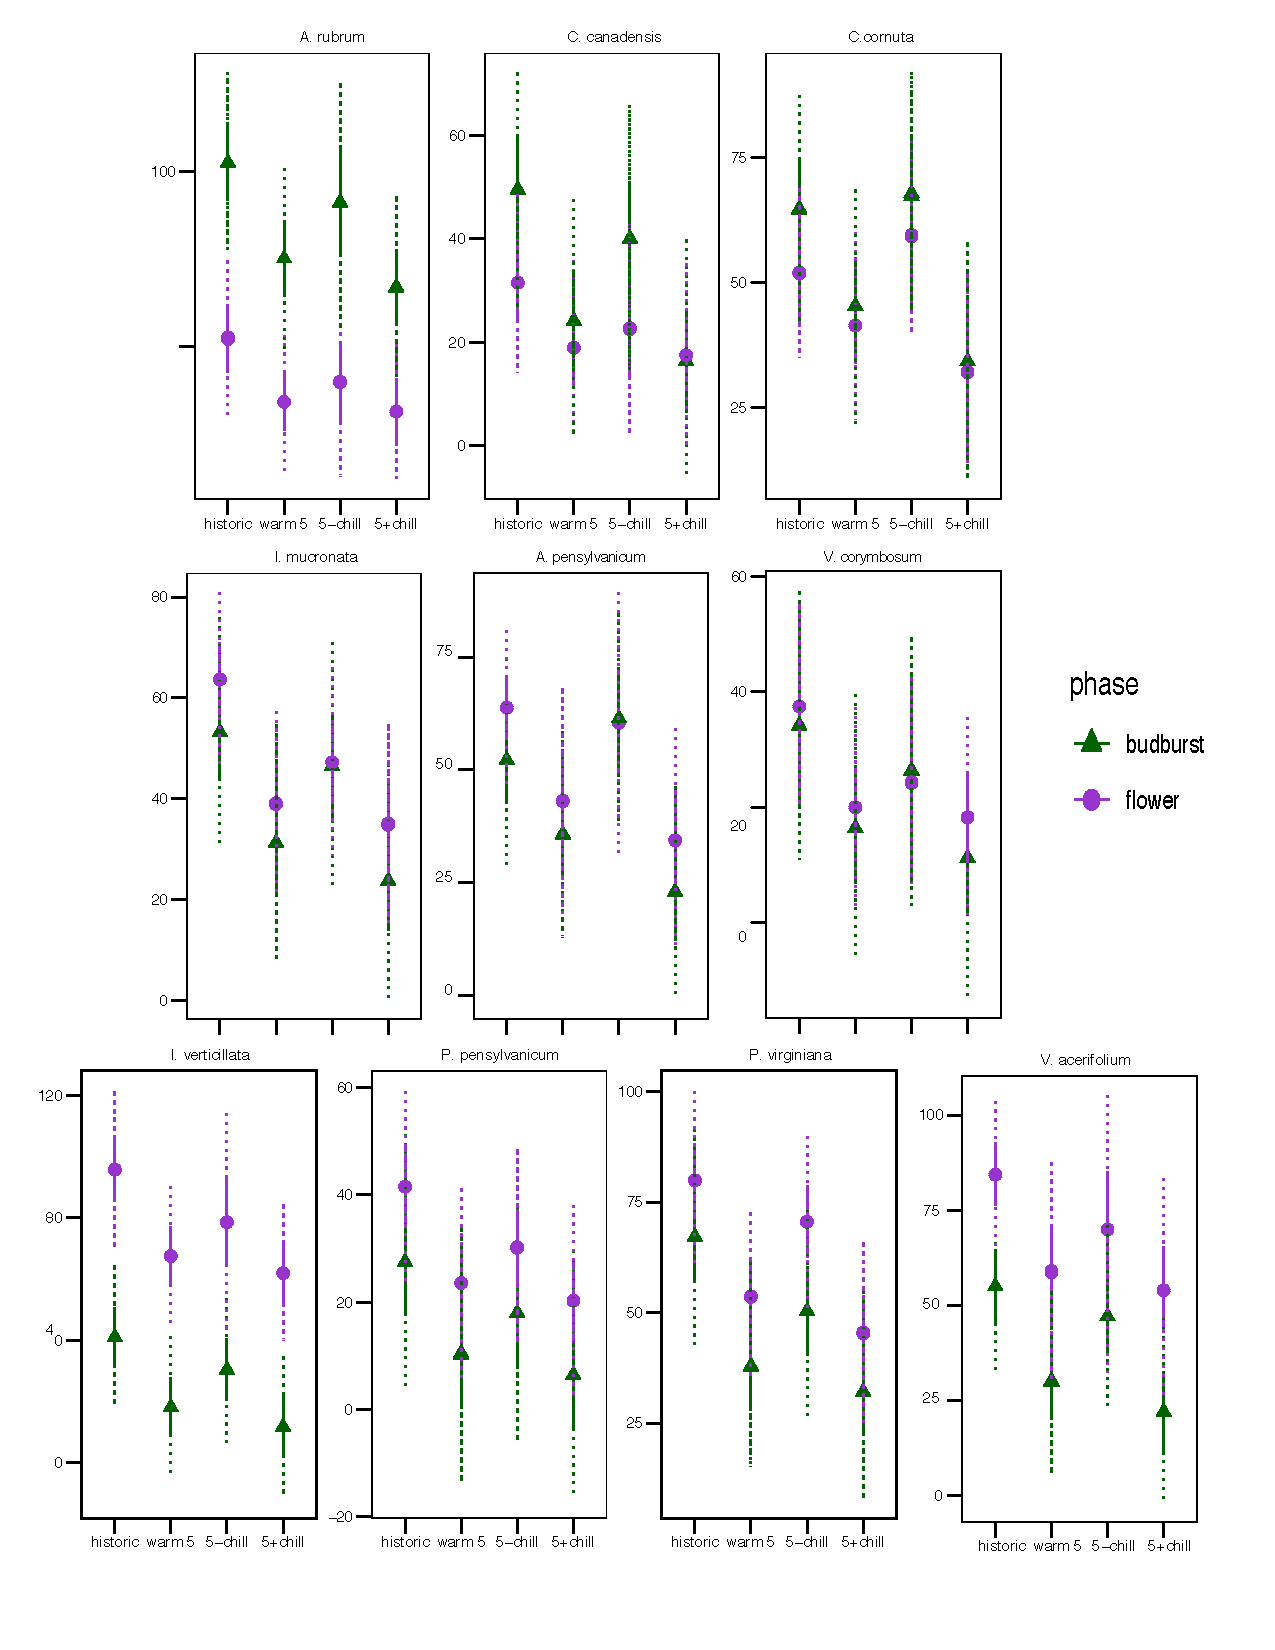
\includegraphics[width=\textwidth]{..//Plots/Flobuds_manuscript_figs/climpredictions.pdf}
    \caption{This shows our climate change predictions }
    \label{fig:preddy}
\end{figure}


\begin{figure}[h!]
    \centering
 \includegraphics[width=\textwidth]{..//Plots/Flobuds_manuscript_figs/raw_plots_final.pdf}
    \caption{\textbf{This figure need to be re-made using bbch 9 instead of 15, but should probably just show vaccinium or bounce to supplement}}
    \label{fig:raw}
    \end{figure}

\begin{figure}[h!]
    \centering
 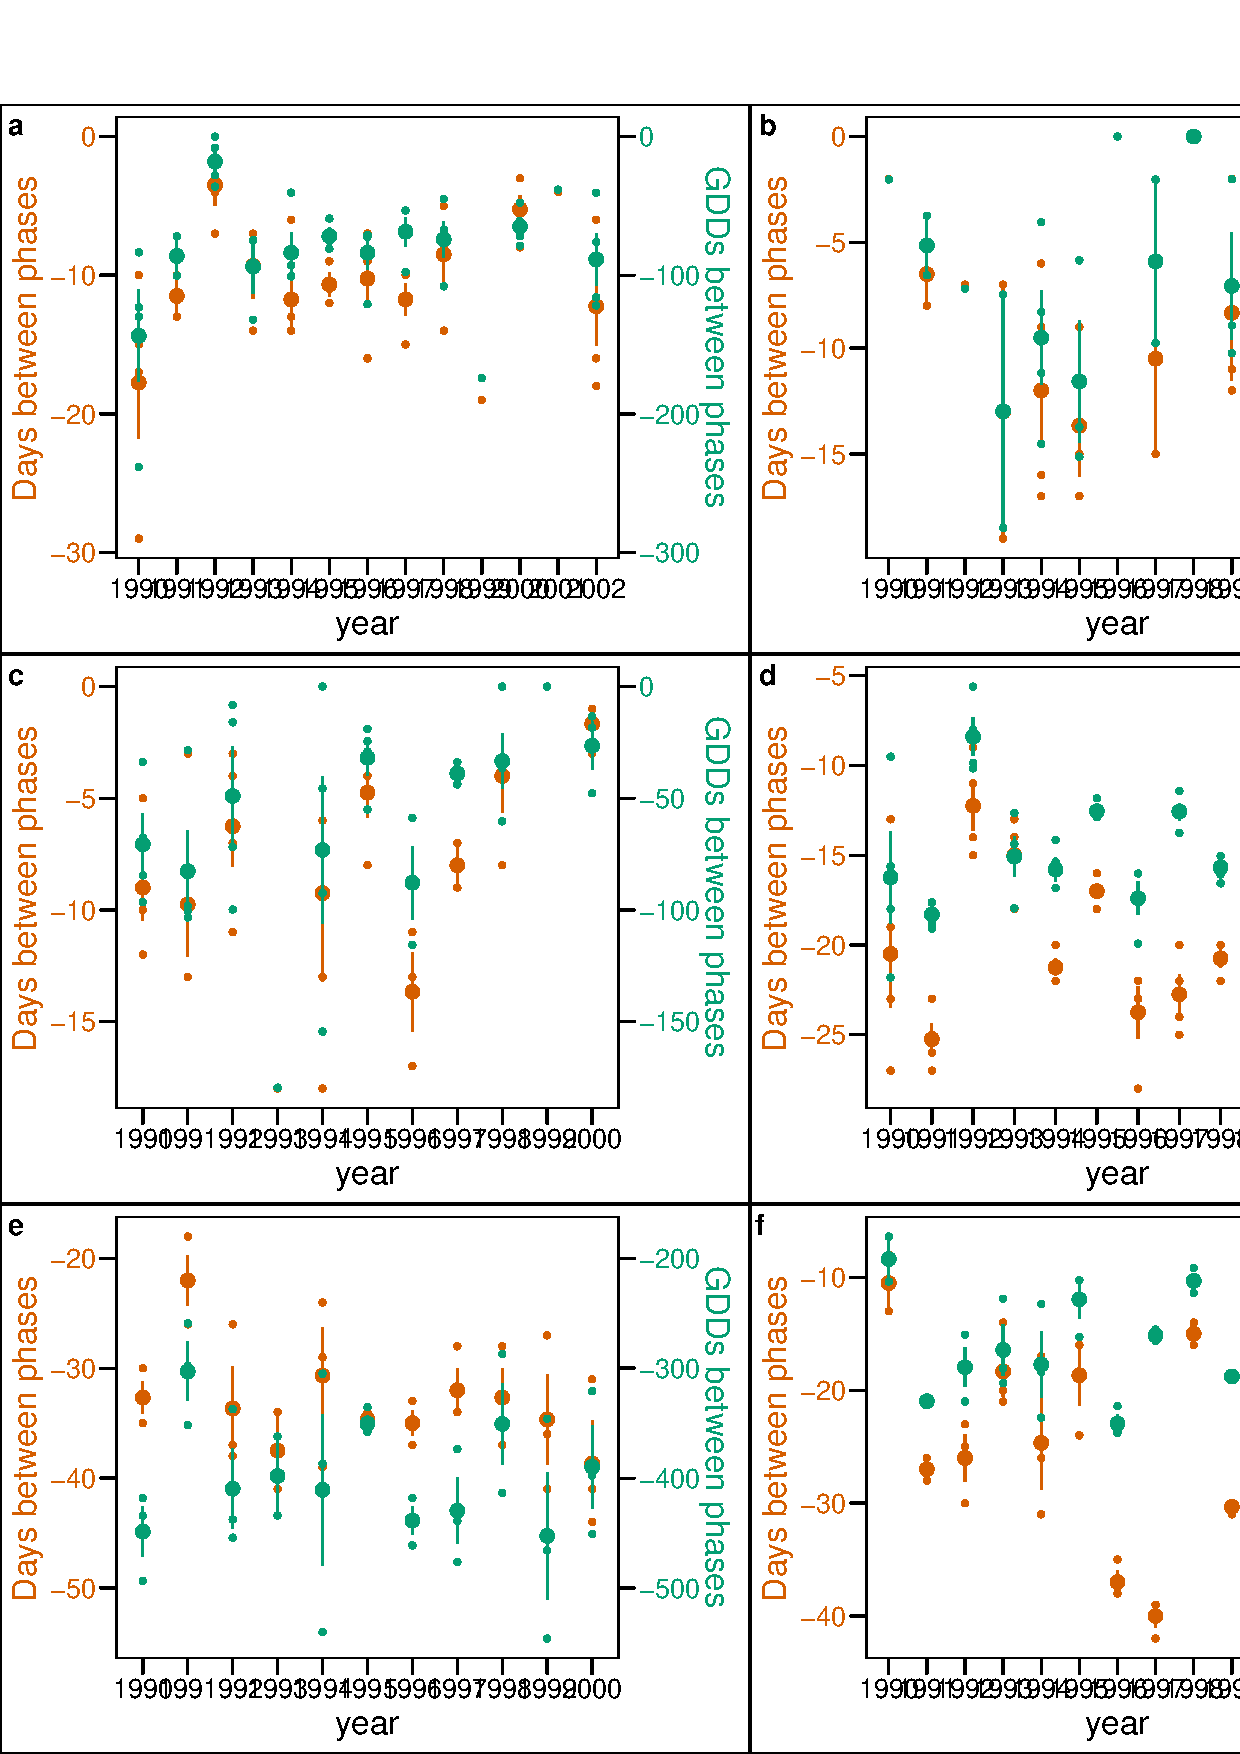
\includegraphics[width=\textwidth]{..//Plots/supp_field_sps.jpeg}
    \caption{\textbf{Other species in HF}}
    \label{fig:other}
    \end{figure}

\end{document}